\section{Description générale de l'existant}

\subsection{Le Sokoban original}
Sokoban est un jeu vidéo japonais de type puzzle sorti en 1986. Le but est de déplacer des caisses à des emplacements précis en les poussant grâce à notre petit personnage. Une fois toutes les caisses en place le niveau s'achève et un nouveau 
commence.

\begin{figure}[h]
	\centering
	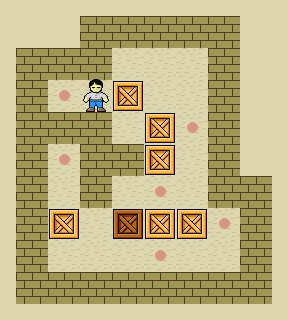
\includegraphics {Sokoban.jpg}
	\caption{Sokoban original de 1986}
	\label{fig:Sokoban_original}
\end{figure}

\subsection{Slimoban}
Slimoban est un jeu dérivé du Sokoban original, dans cette version, il s'agit toujours d'un jeu de puzzle mais cette fois, le but est de récupérer une pièce d'or en résolvant les énigmes jusqu'à la pièce d'or.

\begin{figure}[h]
	\centering
	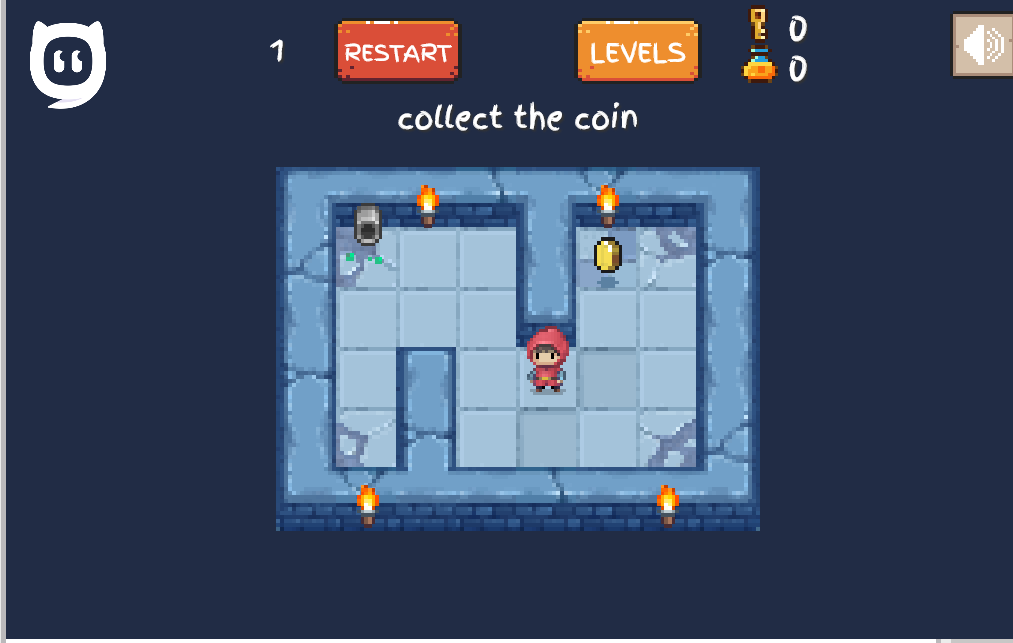
\includegraphics[width=0.5\textwidth]{slimoban.png}
	\caption{Slimoban}
	\label{fig:slimoban}
\end{figure}

\newpage
\subsection{BlupiMania}
BlupiMania est également un jeu dérivé du Sokoban original mais dans celui-ci, le jeu est en 3D, de plus le jeu est agrémenté de nouveaux objets (tels que des accélérateurs, détonateurs, des trous, \ldots) modifiant ainsi la façon de jouer.

\begin{figure}[h]
	\centering
	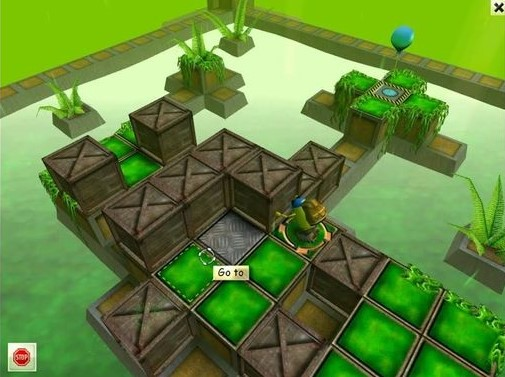
\includegraphics[width=0.5\textwidth] {blupimania.jpg}
	\caption{BlupiMania}
	\label{fig:blupimania}
\end{figure}